\chapter{The Standard Model of Cosmology}
\label{chap:the-standard-model-of-cosmology}
\thispagestyle{empty}

\noindent The standard model of cosmology describes an expanding universe. Its basic assumptions are that the cosmological principle is valid and that general relativity can describe nature on cosmological scales. \\

\noindent The dynamics of the expansion is guided by the cosmological constant $\Lambda$ in Einstein's field equations, since this term was initally introduced to act repulsive towards gravity, so that the universe does not collapse due to the gravity of matter it contains. The drive behind the \textit{accelerated} expansion was given the name ``dark energy'', which refers in the $\Lambda$CDM-model to the cosmological constant $\Lambda$. \\ 
Nevertheless, it should be mentioned that the term ``dark energy'' used in cosmology is not restricted to the cosmological constant. Its meaning depends on the particular cosmological model that is considered (see subsection 2.4.6 ``\textit{Dark energy}'' in \cite[p.~50]{Dodelson2020} and \cite{Frieman2008}). \\

\noindent The ``CDM`` in ``$\Lambda$CDM'' stands for ``cold dark matter''. There are several indications that lead to the assumption of the existence of dark matter. The first and probably most dominant indication is by observing the velocity of stars while surrounding their galactic center. While, according to classical mechanics, the rotation velocity of an object in a gravitational field should decrease the further the object is to the center of mass, it is observed that the rotation curve (the distance-velocity-relation, see \cite[p.~64]{Schneider2006}) in spiral galaxies does not decrease, which leads to the assumption that there has to be some mass in galactic halos that holds the galactic disk together due to its gravity (otherwise, galaxies should fall apart due to the high velocity of the stars that surround the galactic nucleus). \\
Apart from the absence of other interactions than gravitational, dark matter behaves like ordinary (baryonic) matter according to the $\Lambda$CDM-model. While theories on ``hot'' dark matter assume small masses for the particles that dark matter consists of, so that they behave more like relativistic hot gas, the $\Lambda$CDM-model assumes ``cold'' dark matter, which means in this context heavy particles that behave more classically. \\

\noindent For the purpose of this thesis, the distinction between ordinary, baryonic matter and dark matter can be neglected.



\section{The Cosmological Principle}

The cosmological principle states that, assuming the universe does not prefer any direction in space, i.e. the universe is isotropic for \textit{every} observer, the larger scales we consider, the smaller the variance and thus the more homogeneous the matter distribution appears. \\
A more mathematically rigorous definition of the cosmological principle can be found in \cite[p.~5]{Bartelmann2019} and \cite[p.~713/714]{MTW2017}.
\begin{figure}[H]
    \centering
    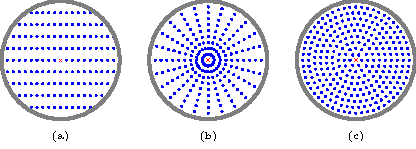
\includegraphics[scale=2.2]{figures/tikz/homogeneous-isotropic/homogeneous-isotropic}
    \caption{The cosmological principle visualized. \\
    The matter distribution (a) is homogeneous, but not isotropic. \\
    The matter distribution (b) is for an observer at the center isotropic, but not homogeneous. \\
    The matter distribution (c) is for an observer at the center isotropic \textit{and} homogeneous.}
    \label{fig:homogeneous-isotropic}
\end{figure}
\noindent Obviously, the universe is not perfectly homogeneous (especially not on small scales, for example our galactic neighborhood), but keep in mind that the cosmological principle does \textit{not} postulate a perfect homogeneous and isotropic universe. \\
Instead, the cosmological principle is a statement about the \textit{statistics} of matter distribution. \\
The \textit{larger} the scales an observer considers at \textit{any} point in the universe, the \textit{more} homogeneous the matter distribution appears. \\

\noindent The strongest evidence at current state that supports the cosmological principle is the measurement of the cosmic microwave background, whose radiation spectrum follows the Planck distribution of a black body radiator with $T \approx \SI{2.736}{\kelvin}$ more accurately than any other measurement in nature (\cite[p.~131/132]{Peebles1993} and \cite{White1999}). 

\begin{figure}[H]
    \centering
    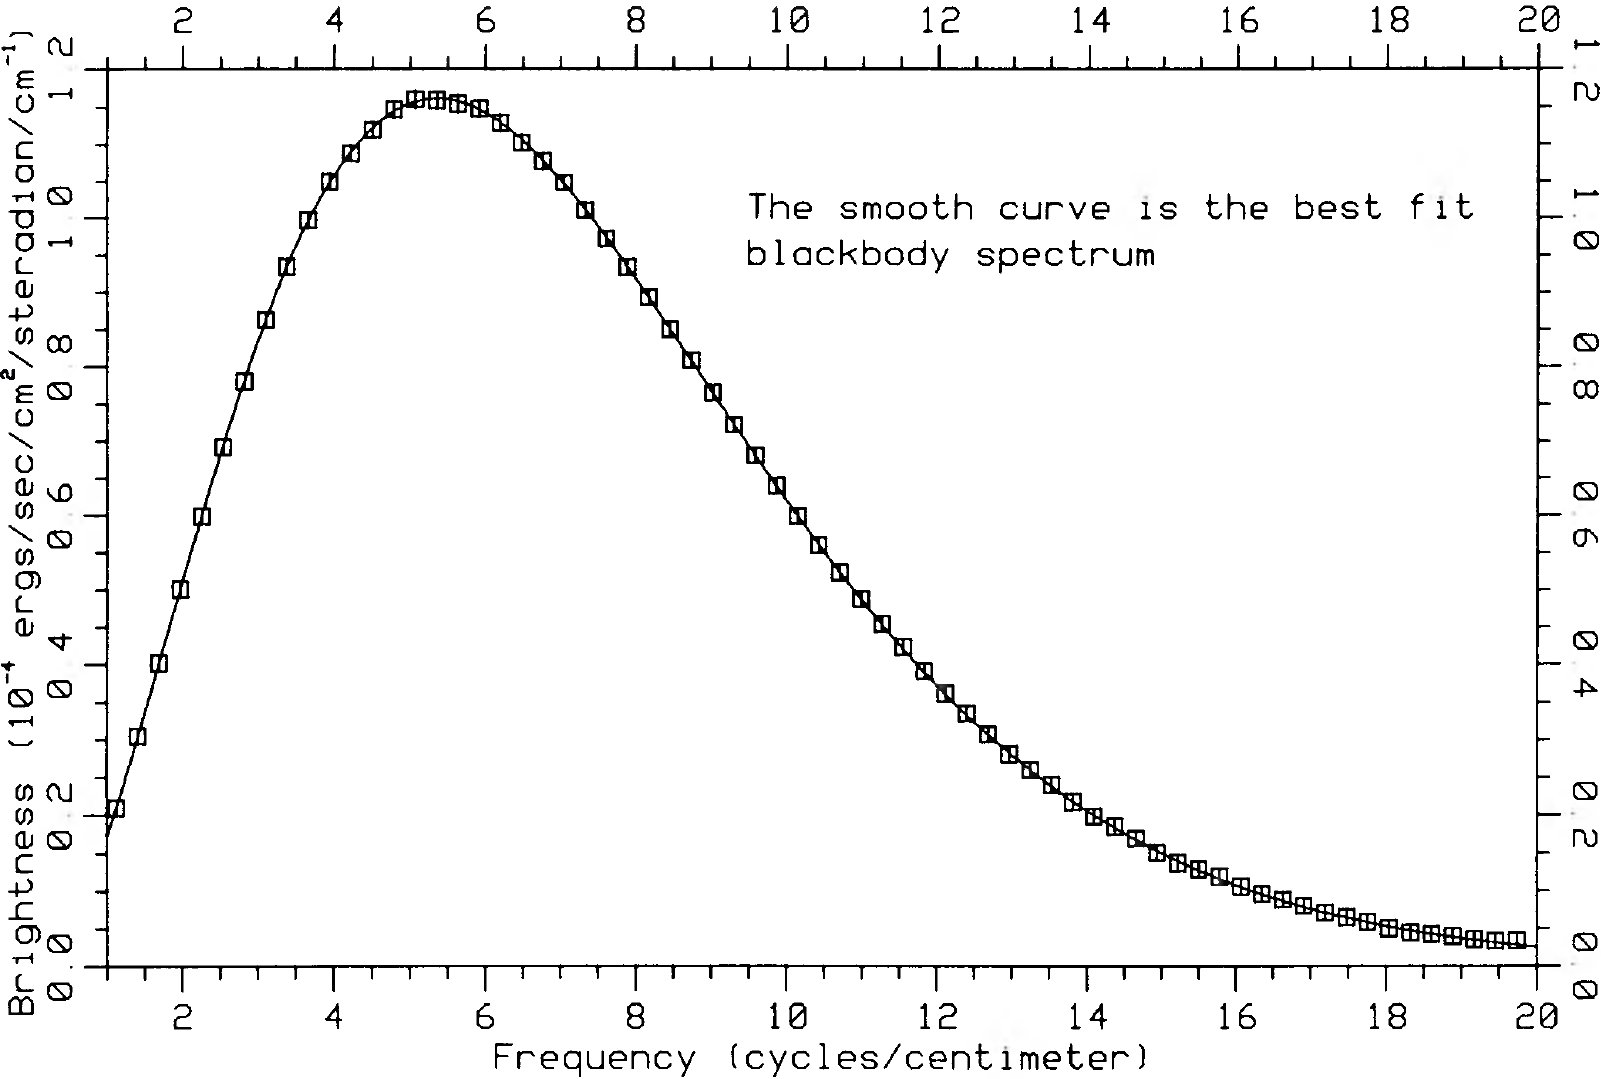
\includegraphics[scale=0.34]{figures/images/cmb-blackbody.png}
    \caption[Caption for LOF]{The spectrum of the microwave background radiation, measured by ``COBE'' (Cosmic Background Explorer) in 1990. For this exploration, John C. Mather and George F. Smoot were awarded the Nobel Prize in Physics in 2006. \\
    Source: \cite[Figure 2]{Mather1990}}
\end{figure}


\subsection{FLRW-Metric}

Motivated by the cosmological principle, there are mathematically three possible geometries for the four-dimensional spacetime that satisfy spatial homogeneity and isotropy of the metric:
\begin{itemize}
    \item a four-dimensional sphere $\mathcal{S}^{3}$ with positive curvature,
    \item a four-dimensional flat space $\mathcal{F}^{3}$ with zero curvature,
    \item a four-dimensional hyperboloid $\mathcal{H}^{3}$ with negative curvature.
\end{itemize}

\noindent We can parameterize these geometries by
\begin{align}
    \begin{pmatrix} x \\ y \\ z \\ w \end{pmatrix} &\overset{\mathcal{S}^{3}}{=} \begin{pmatrix} \sin(\psi) \sin(\theta) \cos(\phi) \\ \sin(\psi) \sin(\theta) \sin(\phi) \\ \sin(\psi) \cos(\theta) \\ \cos(\psi) \end{pmatrix} \overset{\mathcal{F}^{3}}{=} \begin{pmatrix}  \psi \sin(\theta) \cos(\phi) \\ \psi \sin(\theta) \sin(\phi) \\ \psi \cos(\theta) \\ 1 \end{pmatrix} \overset{\mathcal{H}^3}{=} \begin{pmatrix} \sinh(\psi) \sin(\theta) \cos(\phi) \\ \sinh(\psi) \sin(\theta) \sin(\phi) \\ \sinh(\psi) \cos(\theta) \\ \cosh(\psi) \end{pmatrix} \nonumber \\
                                                   &= \begin{pmatrix} r \sin(\theta) \cos(\phi) \\ r \sin(\theta) \sin(\phi) \\ r \cos(\theta) \\ \pdv{r}{\psi} \end{pmatrix} \quad \text{with} \quad r = \begin{cases} \sin(\psi) \quad &\text{for} \quad \mathcal{S}^{3} \\ \psi \quad &\text{for} \quad \mathcal{F}^{3} \\ \sinh(\psi) \quad &\text{for} \quad \mathcal{H}^{3} \end{cases}. \label{eq:geometry}
\end{align}

\noindent The metric for the spatial line element $\dd{\ell}$ is 
\begin{align}
    \dd{\ell}^2 = \begin{cases} 
                    \dd{x}^2 + \dd{y}^2 + \dd{z}^2 + \dd{w}^2 \quad &\text{for} \quad \mathcal{S}^{3} \\ 
                    \dd{x}^2 + \dd{y}^2 + \dd{z}^2 \quad &\text{for} \quad \mathcal{F}^{3} \\ 
                    \dd{x}^2 + \dd{y}^2 + \dd{z}^2 - \dd{w}^{2} \quad &\text{for} \quad \mathcal{H}^{3} 
                  \end{cases}. \label{eq:spatial-metric}
\end{align}

\noindent With the parameterization in Equation \eqref{eq:geometry}, we can write for the infinitesimals 
\begin{align*}
    \dd{x} &= \sin(\theta) \cos(\phi) \dd{r} + r \cos(\theta) \cos(\phi) \dd{\theta} - r \sin(\theta) \sin(\phi) \dd{\phi}, \nonumber \\
    \dd{y} &= \sin(\theta) \sin(\phi) \dd{r} + r \cos(\theta) \sin(\phi) \dd{\theta} + r \sin(\theta) \cos(\phi) \dd{\phi}, \nonumber \\
    \dd{z} &= \cos(\theta) \dd{r} - r \sin(\theta) \dd{\theta}, \nonumber \\
    \dd{w} &= \pdv{w}{r} \dd{r} = \pdv{}{r} \biggl(\pdv{r}{\psi}\biggr) \dd{r} \nonumber.
\end{align*}

\noindent The components $\dd{x}$, $\dd{y}$ and $\dd{z}$ lead to 
\begin{align*}
    \dd{x}^2 + \dd{y}^2 + \dd{z}^2 = \dd{r}^2 + r^2 \bigl[ \underbrace{\dd{\theta}^2 + \sin^2(\theta) \dd{\phi}^2}_{=: \dd{\Omega}^2} \bigr] = \dd{r}^2 + r^2 \dd{\Omega}^2,
\end{align*}
where $\dd{\Omega}$ is the infinitesimal spatial angle. \\
Let us have a closer look on $\dd{w}$. We obtain
\begin{align}
    \dd{w} = \dd{r} \begin{cases} 
                        \pdv{}{r} \cos(\psi) = \pdv{}{r} \cos(\arcsin(r)) = -\frac{r}{\sqrt{1 - r^2}} \quad &\text{for} \quad \mathcal{S}^{3} \\
                        \pdv{}{r} 1 = 0 \quad &\text{for} \quad \mathcal{F}^{3} \\
                        \pdv{}{r} \cosh(\psi) = \pdv{}{r} \cosh(\arsinh(r)) = \frac{r}{\sqrt{1 + r^2}} \quad &\text{for} \quad \mathcal{H}^{3}
                    \end{cases}, 
\end{align}
and hence for the spatial component of the metric \eqref{eq:spatial-metric}
\begin{align}
    \dd{\ell}^2 = \begin{cases}
                      \frac{1}{1 - r^2} \dd{r}^2 + r^2 \dd{\Omega}^2 \quad &\text{for} \quad \mathcal{S}^{3} \\
                      \dd{r}^2 + r^2 \dd{\Omega}^2 \quad &\text{for} \quad \mathcal{F}^{3} \\
                      \frac{1}{1 + r^2} \dd{r}^2 + r^2 \dd{\Omega}^2 \quad &\text{for} \quad \mathcal{H}^{3}
                  \end{cases}. \label{eq:spatial-metric-cases}
\end{align}
If we define 
\begin{align}
    k := \begin{cases}
            1 \quad &\text{for} \quad \mathcal{S}^{3} \\
            0 \quad &\text{for} \quad \mathcal{F}^{3} \\
            -1 \quad &\text{for} \quad \mathcal{H}^{3} \\
         \end{cases}, 
\end{align}
we can write Equation \eqref{eq:spatial-metric-cases} in compact notation as 
\begin{align}
    \dd{\ell}^2 = \frac{1}{1 - k r^2} \dd{r}^2 + r^2 \dd{\Omega}^2. 
\end{align}
Since the cosmological model describes an expanding universe, we introduce the scale factor $a(t)$, by which the spatial line element $\dd{\ell}$ is scaled at time $t$. \\
Therefore, we finally obtain the Friedmann--Lemaître--Robertson--Walker metric of spacetime
\begin{align}
    \dd{s}^2 = - c^2 \dd{t}^2 + a^2(t) \dd{\ell}^2 = - c^2 \dd{t}^2 + a^2(t) \biggl[\frac{1}{1 - k r^2} \dd{r}^2 + r^2 \dd{\Omega}^2 \biggr]. \label{eq:FLRW-metric}
\end{align}



\section{Friedmann Equations}

Applying the FLRW-metric to Einstein's field equations leads to the fundamental equations -- the Friedmann equations -- that describe the dynamics of the expansion of the universe by the scale factor $a(t)$ with (\cite[p.~11]{Bartelmann2019})
\begin{align}
    \biggl(\frac{\dot{a}}{a}\biggr)^2 &= \frac{8\pi G}{3} \rho - \frac{k c^2}{a^2} + \frac{\Lambda c^2}{3} , \label{eq:friedmann1} \\
    \frac{\ddot{a}}{a} &= -\frac{4\pi G}{3}\biggl( \rho + \frac{3p}{c^2}\biggr) + \frac{\Lambda c^2}{3} \label{eq:friedmann2}.
\end{align}
Those equations contain the energy density $\rho(t) = \rho_{\text{m}}(t) + \rho_{\text{r}}(t)$ of matter and radiation, the curvature parameter $k$ of the FLRW-metric, the pressure $p$ that matter and radiation exerts as a perfect fluid and the cosmological constant $\Lambda$. \\

\noindent Taking the derivative of Equation \eqref{eq:friedmann1} with respect to time and inserting into Equation \eqref{eq:friedmann2} leads to the differential equation 
\begin{align}
    \dot{\rho} + 3\frac{\dot{a}}{a} \biggl( \rho + \frac{p}{c^2} \biggr) = 0. \label{eq:friedmann3}
\end{align}
We define the Hubble parameter $\displaystyle H(t):= \frac{\dot{a}}{a}$ and $\displaystyle w := \frac{p}{\rho c^2}$, which leads with Equation \eqref{eq:friedmann3} to 
\begin{align}
    \dot{\rho} + 3H\rho(1+w) = 0. \label{eq:friedmann-continuity-equation}  
\end{align}
This Equation \eqref{eq:friedmann-continuity-equation} is sometimes called ``the continuity equation of cosmology''. We obtain by integration the relation between density $\rho(t)$ and scale factor $a(t)$ 
\begin{align}
    \rho(a) = \rho_{0} a^{-3(1 + w)}(t) \label{eq:density-scale-factor-relation} 
\end{align}
with $\rho_{0} := \rho(a(t_{0}))$.


\subsection{Density Parameters}

\noindent We are now interested in how the density components of the universe change as a function of the expansion of the universe scaled by $a(t)$. \\

\noindent In the case of matter at rest, the density of matter $\rho_{\text{m}}$ shrinks by $a^{3}(t)$ when the volume that contains the matter is scaled by $a(t)$, so 
\begin{align}
    \rho_{\text{m}}(a) = \frac{E}{V(a)} = \frac{E}{V_{0} a^{3}(t)} = \rho_{\text{m}, 0} a^{-3}(t). \label{eq:matter-density-scale} 
\end{align}
With comparison to Equation \eqref{eq:density-scale-factor-relation} follows $w_{\text{m}} = 0$.

\noindent In the case of radiation, we have to account that its wavelength $\lambda$ is scaled by the factor $a(t)$, so $\lambda(a) = \lambda_{0} a(t)$, which leads with $E(\lambda) = h c / \lambda$ to the energy density

\begin{align}
    \rho_{\text{r}}(a) = \frac{E(a)}{V(a)} = \frac{1}{V_{0} a^3(t)} \frac{h c}{\lambda_{0} a(t)} = \frac{h c}{V_{0} \lambda_{0}} \frac{1}{a^{4}(t)} = \rho_{\text{r},0} a^{-4}(t). \label{eq:radiation-density-scale}
\end{align}
With comparison to Equation \eqref{eq:density-scale-factor-relation} follows $w_{\text{r}} = \frac{1}{3}$.

\noindent Now, let us rewrite the cosmological constant $\Lambda$ by defining
\begin{align}
    \rho_{\Lambda} := \frac{\Lambda c^2}{8\pi G}
\end{align}
as the density that relates to the cosmological constant. As the name might imply, this density remains constant as the universe expands and is therefore independent of the scale factor $a(t)$.
This interpretation of $\Lambda$ leads to the assumption, that $\rho_{\Lambda}$ can be viewed as the energy density of vacuum. As vacuum increases exact the same way as space expands, its density remains constant, so
\begin{align}
    \rho_{\Lambda}(a) = \rho_{\Lambda,0}. \label{eq:lambda-density-scale}
\end{align}
With comparison to Equation \eqref{eq:density-scale-factor-relation} follows $w_{\Lambda} = -1$.

\noindent Our aim is now to write Equation \eqref{eq:friedmann1} as a sum of densities. We therefore define a ``density'' that would relate to the spatial curvature $k$,
\begin{align}
    \rho_{k} := -\frac{3}{8 \pi G} kc^2 a^{-2}(t). \label{eq:curvature-density-scale}
\end{align}
Further, we define the critical density $\rho_{\text{cr}}$ as the density the universe would have if it was flat ($k=0$) and had no component of $\Lambda$ at the time $t_{0}$, so with $H_{0} := H(t_{0})$
\begin{align}
    \rho_{\text{cr}} := \frac{3 H_{0}^2}{8\pi G}. \label{eq:critical-density} 
\end{align}
Finally, we define 
\begin{align}
    \Omega_{i} := \frac{\rho_{i}}{\rho_{\text{cr}}} \label{eq:normalized-density}
\end{align}
where $i$ is the label for the density type. We can then write Equation \eqref{eq:friedmann1} as 
\begin{align}
    H^{2}(t) &= \frac{8\pi G}{3} \rho_{\text{r+m}} - \frac{kc^2}{a^2} + \frac{\Lambda c^2}{3} \nonumber \\
             &= \frac{8 \pi G}{3} \bigl( \rho_{\text{r}} + \rho_{\text{m}} + \rho_{k} + \rho_{\Lambda} \bigr) \nonumber \\     
             &= H_{0}^{2} \frac{1}{\rho_{\text{cr}}} \bigl( \rho_{\text{r}} + \rho_{\text{m}} + \rho_{k} + \rho_{\Lambda} \bigr) \nonumber \\
             &= H_{0}^{2} \sum_{i \in \{\text{r}, \text{m}, k, \Lambda \}} \Omega_{i}. \label{eq:hubble-square}
\end{align}
We clearly see that the sum of all normalized density parameters $\Omega_{i,0}$ at time $t_{0}$ lead to
\begin{align}
    1 = \Omega_{\text{r},0} + \Omega_{\text{m},0} + \Omega_{k,0} + \Omega_{\Lambda, 0}. \label{eq:density-parameters-sum} 
\end{align}
With the relations \eqref{eq:matter-density-scale}, \eqref{eq:radiation-density-scale}, \eqref{eq:lambda-density-scale}, \eqref{eq:curvature-density-scale} between the densities and the scale factor, we obtain
\begin{align*}
    H^{2}(t) &= \frac{8 \pi G}{3} \bigl(\rho_{\text{r}} + \rho_{\text{m}} + \rho_{k} + \rho_{\Lambda} \bigr) \\
             &= H_{0}^{2} \frac{1}{\rho_{\text{cr}}} \bigl(\rho_{\text{r},0} a^{-4}(t) + \rho_{\text{m},0} a^{-3}(t) + \rho_{\text{k},0} a^{-2}(t) + \rho_{\Lambda,0} \bigr) \\
             &= H_{0}^{2} \bigl(\Omega_{\text{r},0} a^{-4}(t) + \Omega_{\text{m},0} a^{-3}(t) + \Omega_{k,0} a^{-2}(t) + \Omega_{\Lambda,0} \bigr) \\
             &=: H_{0}^{2} E^{2}(a),
\end{align*}
and we call 
\begin{align}
    E(a) := \sqrt{\Omega_{\text{r},0} a^{-4}(t) + \Omega_{\text{m},0} a^{-3}(t) + \Omega_{k,0} a^{-2}(t) + \Omega_{\Lambda,0}} \label{eq:expansion-function} 
\end{align}
the expansion function. \\

\noindent With the obtained values by the \textit{Planck Collaboration} (see \cite[Table 7]{Planck2020}), $\Omega_{\text{m},0} \approx 0.3111 \pm 0.0056$, $\Omega_{\text{r},0} = \frac{1}{1 + z_{\text{eq}}} \Omega_{\text{m},0} \approx \SI{9.812e-5}{}$ (at $z_{\text{eq}} = 3387 \pm 21$) and $\Omega_{\Lambda,0} \approx 0.6889 \pm 0.0056$, we see that the radiation component was only relevant in the first $\sim \SI{380000}{\yr}$ of the universe until matter and radiation decoupled.

\begin{figure}[H]
    \centering
    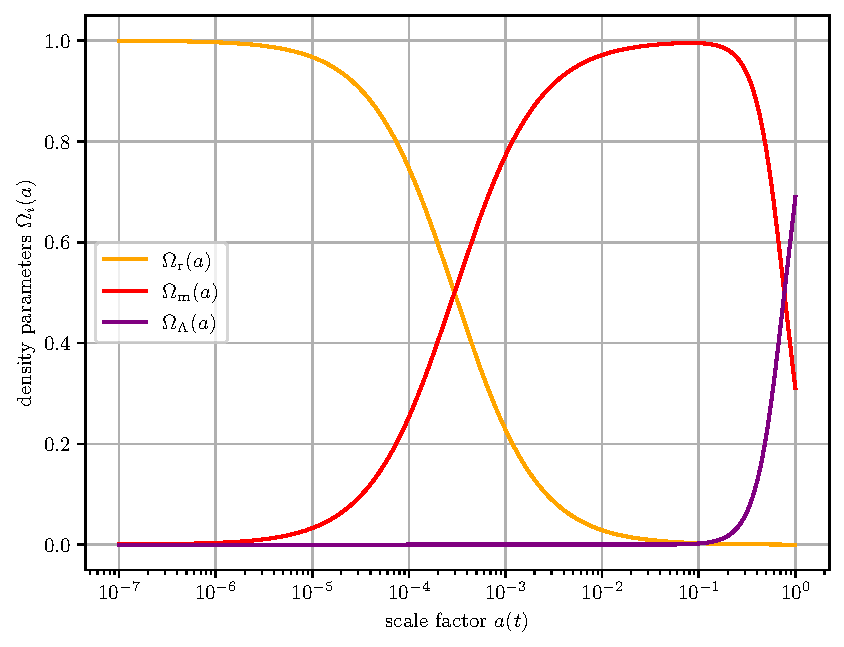
\includegraphics[scale=1.0]{figures/plots/PDF/scale-factor-vs-density-parameters}
    \caption{The normalized density parameters of radiation, matter and $\Lambda$ in dependence of the scale factor $a(t)$ on logarithmic axis.}
    \label{fig:scale-factor-vs-density-parameters}
\end{figure}

\noindent Since the radiation does not contribute significantly to the expansion of the universe, we assume for the rest of this thesis $\Omega_{\text{r},0} = 0$. \label{no-radiation} \\
Further, the universe appears to be almost flat (\cite[Table 7]{Planck2020}) with a measured value of $\Omega_{k,0} \approx 0.0007 \pm 0.0019$. 

\noindent Let us have a look how $\Omega_{\text{m},0}$ and $\Omega_{\Lambda,0}$ contribute to the expansion of a flat universe. 

\begin{figure}[H]
    \centering
    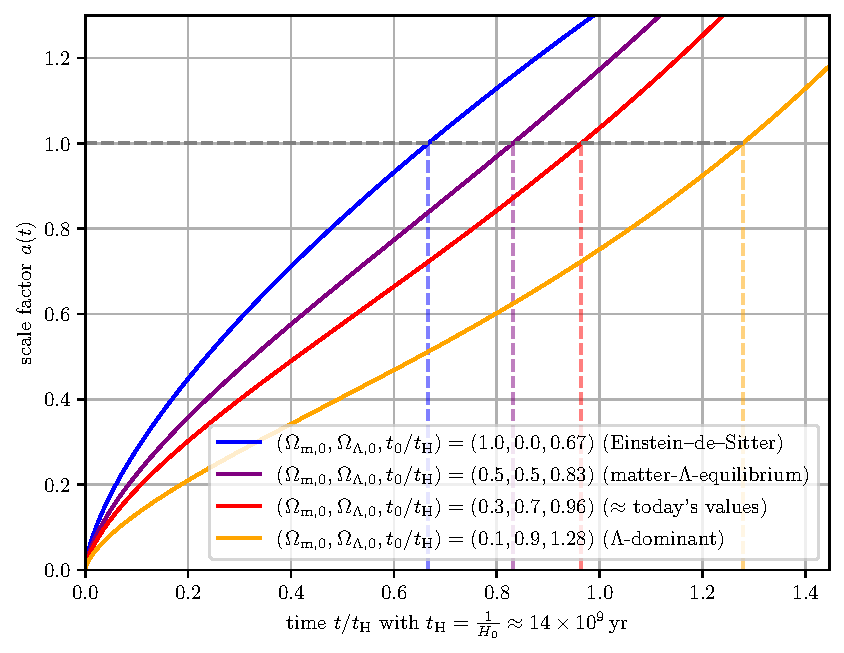
\includegraphics[scale=1.0]{figures/plots/PDF/time-vs-scale-factor}
    \caption{Contribution of $\Omega_{\text{m},0}$ and $\Omega_{\Lambda,0}$ to the expansion in a flat universe ($k = 0$) without radiation $\Omega_{\text{r},0} = 0$ for several cosmologies. $t_{\text{H}} = \frac{1}{H_{0}} \approx \SI{14e+9}{\yr}$ is the Hubble time.}
    \label{fig:time-vs-scale-factor}
\end{figure}

\noindent We notice from Figure \ref{fig:time-vs-scale-factor} that the higher the value of $\Omega_{\Lambda,0}$, the more it contributes to an accelerated expansion. \\

\noindent We define $a(t_{0}) := 1$ as the scale factor at the time $t_{0} =: t_{\text{today}}$. \\
With $\displaystyle \dv{a}{t} = H_{0} a E(a)$, the age of the universe can be calculated by 
\begin{align}
    t_{0} = \frac{1}{H_{0}} \int\limits_{0}^{a(t_{0})} \dd{a} \frac{1}{a E(a)} = \frac{1}{H_{0}} \int\limits_{0}^{1} \dd{a} \frac{1}{\sqrt{\Omega_{\text{r},0} a^{-2} + \Omega_{\text{m},0} a^{-1} + \Omega_{k,0} + \Omega_{\Lambda,0} a^{2}}}. \label{eq:age-of-universe}
\end{align}

\noindent For a flat universe without considering radiation ($\Omega_{k,0} =0$, $\Omega_{\text{r},0} = 0$), the expression \eqref{eq:age-of-universe} can be calculated analytically. With $\Omega_{\text{m},0} = 0.3$ and therefore $\Omega_{\Lambda,0} = 1 - \Omega_{\text{m},0} = 0.7$, we obtain 
\begin{align}
    t_{0} = \frac{2}{3 H_{0} \sqrt{1 - \Omega_{\text{m},0}}} \arsinh \biggl( \sqrt{\frac{1 - \Omega_{\text{m},0}}{\Omega_{\text{m},0}}} a^{\frac{3}{2}}(t_{0}) \biggr) \approx \SI{13.8e+9}{\yr}. 
\end{align}


\newpage
\section{Measures of Distance}

Given the equations the standard model provides, we can derive measures of cosmological distances. \\
As already mentioned, the wavelength of light that travels to an observer is being redshifted due to the expansion of the universe. The relation between the scale factor and the redshift is given by (see \cite[p.~9]{Bartelmann2019})
\begin{align}
    a(z) = \frac{1}{1 + z}. \label{eq:scale-factor-redshift-relation}
\end{align}
For the path that light travels between two points (events) in spacetime (also called ``lightlike geodesics''), we have $\dd{s} = 0$, which leads with the FLRW-metric (see Equation \eqref{eq:FLRW-metric}) and isotropy $(\dd{\Omega} = 0)$ to 
\begin{align}
    - \frac{c}{a(t)} \dd{t} = \frac{1}{\sqrt{1 - kr^2}} \dd{r}. \label{eq:lightlike-path} 
\end{align}
For the left-hand side of Equation \eqref{eq:lightlike-path}, we can write 
\begin{align}
    - \frac{c}{a(t)} \dd{t} = - \frac{c}{a} \frac{1}{\dot{a}} \dd{a} = - \frac{c}{H_{0}} \frac{1}{a^2 E(a)} \dd{a}
\end{align}
and with $\displaystyle \dd{z} = - \frac{1}{a^2} \dd{a}$, 
\begin{align}
    - \frac{c}{a(t)} \dd{t} = - \frac{c}{H_{0}} \frac{1}{a^2 E(a)} \dd{a} = \frac{c}{H_{0}} \frac{1}{E(z)} \dd{z}. \label{eq:RHS-lightlike-path}
\end{align}
We define $\displaystyle d_{\text{H}} := \frac{c}{H_{0}}$ as the \text{Hubble distance}. \\
For the right-hand side of Equation \eqref{eq:lightlike-path}, we obtain for the integration
\begin{align}
    \int\limits_{0}^{d_{\text{C}}} \frac{1}{\sqrt{1 - kr^2}} \dd{r} =: S^{-1}_{k}(d_{\text{C}}) = \begin{cases} \frac{1}{\sqrt{k}} \arcsin \bigl( \sqrt{k} d_{\text{C}} \bigr) &\text{for} \quad k > 0 \\ d_{\text{C}} &\text{for} \quad k = 0 \\ \frac{1}{\sqrt{\vert k \vert}} \arsinh \bigl(\sqrt{\vert k \vert} d_{\text{C}} \bigr) &\text{for} \quad k < 0 \end{cases}.
\end{align}
The substitution $\displaystyle -k = \frac{1}{d_{\text{H}}^{2}}\Omega_{k,0}$ (see Equations \eqref{eq:curvature-density-scale} and \eqref{eq:critical-density}) leads to
\begin{align}
    S^{-1}_{k} \bigl( \tfrac{d_{\text{C}}}{d_{\text{H}}} \bigr) = d_{\text{H}} \cdot \begin{cases} 
                                                                                        \frac{1}{\sqrt{\vert \Omega_{k,0} \vert}} \arcsin \bigl(\sqrt{\vert \Omega_{k,0} \vert} \frac{d_{\text{C}}}{d_{\text{H}}} \bigr) &\text{for} \quad \Omega_{k,0} < 0  \\ 
                                                                                        \frac{d_{\text{C}}}{d_{\text{H}}} &\text{for} \quad \Omega_{k,0} = 0 \\ 
                                                                                        \frac{1}{\sqrt{\Omega_{k,0}}} \arsinh \bigl(\sqrt{\Omega_{k,0}} \frac{d_{\text{C}}}{d_{\text{H}}}\bigr) &\text{for} \quad \Omega_{k,0} > 0 
                                                                                                                                                                                               \end{cases}. \label{eq:LHS-lightlike-path}
\end{align}
By integration of Equation \eqref{eq:RHS-lightlike-path} follows finally\footnote{I have explicitly performed this derivation, since Equations \eqref{eq:comoving-distance} and \eqref{eq:expansion-integral} are essential for the evaluation of supernovae data and implementation in the source codes in this thesis.}
\begin{align}
    d_{\text{C}} = S_{k}(I) = d_{\text{H}} \cdot \begin{cases} 
                                                    \frac{1}{\sqrt{\vert \Omega_{k,0} \vert}} \sin \bigl(\sqrt{\vert \Omega_{k,0} \vert} I \bigr) &\text{for} \quad \Omega_{k,0} < 0 \\ 
                                                    I &\text{for} \quad \Omega_{k,0} = 0 \\  
                                                \frac{1}{\sqrt{\Omega_{k,0}}} \sinh \bigl(\sqrt{\Omega_{k,0}} I \bigr)  &\text{for} \quad \Omega_{k,0} > 0 
                                                \end{cases} \label{eq:comoving-distance} 
\end{align}
with 
\begin{align}
    I := \int\limits_{0}^{z} \dd{z'} \frac{1}{E(z')}. \label{eq:expansion-integral}  
\end{align}
We call $d_{\text{C}}$ the \textit{comoving distance}.
We define 
\begin{align}
    d_{\text{A}} := \frac{1}{1+z} d_{\text{C}} \label{eq:angular-diameter-distance}
\end{align}
as the \textit{angular diameter distance} and 
\begin{align}
    d_{\text{L}} := (1 + z) d_{\text{C}} \label{eq:luminosity-distance}
\end{align}
as the \textit{luminosity distance}.

\begin{figure}[H]
    \centering
    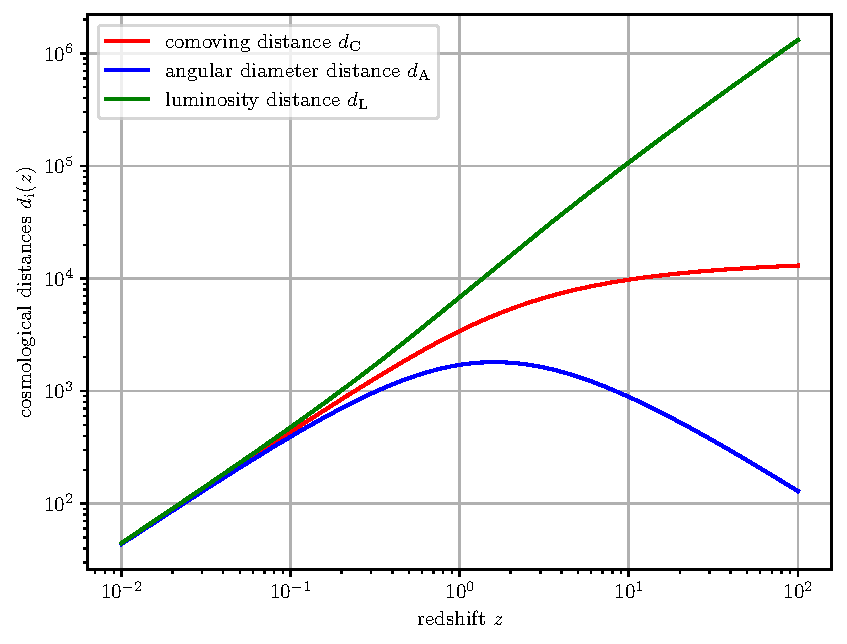
\includegraphics[scale=0.9]{figures/plots/PDF/redshift-vs-cosmological-distances.pdf}
    \caption{Comoving distance $d_{\text{C}}$, angular diameter distance $d_{\text{A}}$ and luminosity distance $d_{\text{L}}$ with respect to redshift $z$ (logarithmic axis) for the $\Lambda$CDM-model with $\Omega_{\text{m},0} = 0.3$, $\Omega_{\Lambda,0} = 0.7$ and $H_{0} = \SI{67.66}{\frac{\kilo \meter}{\second} \mega \parsec^{-1}}$.}
    \label{fig:redshift-vs-cosmological-distances}
\end{figure}

\noindent We can clearly see in Figure \ref{fig:redshift-vs-cosmological-distances} the linear approximation for low redshifts, which explains the linear relation \eqref{eq:lum-dist-approx} that Edwin Hubble observed. Further, we see that those distances require observations at high redshift to distinguish them from each other. \\
The fact of the observed relation $\displaystyle d_{\text{L}}/d_{\text{A}} = (1 + z)^2$ (\cite[p.~58]{Weinberg2008}) and the mentioned slightly broadened light curve of supernovae type Ia due to the slowed supernovae explosion by the factor of $1 + z$ (\cite[p.~10/11]{Goldhaber2001}) shows that the observed redshift is due to an expansion of space,\footnote{Therefore, interpretations of observed redshift due to loss of energy by the received light in a static universe (``tired light''-theory) can be considered as ruled out.} which supports the $\Lambda$CDM-model. \\
\noindent For this thesis, the most relevant distance is the luminosity distance $d_{\text{L}}$.
